% Hlavicka pro protokoly z fyzikalniho praktika.
% Verze pro: LaTeX
% Verze hlavicky: 22. 2. 2007
% Autor: Ustav fyziky kondenzovanych latek
% Ke stazeni: www.physics.muni.cz/ufkl/Vyuka/
% Licence: volne k pouziti, nejlepe k vcasnemu odevzdani protokolu z Vaseho mereni.


\documentclass[czech,11pt,a4paper]{article}
\usepackage[T1]{fontenc}
\usepackage{graphicx}
\usepackage{mathtools}
\usepackage{amssymb}
\usepackage{amsthm}
\usepackage{thmtools}
\usepackage{xcolor}
\usepackage{nameref}
\usepackage{babel}
\usepackage{hyperref}
\usepackage{multicol}
\usepackage[export]{adjustbox}
\usepackage{subcaption}
\usepackage{caption}
\usepackage{multirow}
\usepackage{float}
\usepackage{placeins}




%%% Nemente:
\usepackage[margin=2cm]{geometry}
\newtoks\jmenopraktika \newtoks\jmeno \newtoks\datum
\newtoks\obor \newtoks\skupina \newtoks\rocnik \newtoks\semestr
\newtoks\cisloulohy \newtoks\jmenoulohy
\newtoks\tlak \newtoks\teplota \newtoks\vlhkost
%%% Nemente - konec.


%%%%%%%%%%% Doplnte pozadovane polozky:

\jmenopraktika={Fyzikální praktikum 1}  % nahradte jmenem vaseho predmetu
\jmeno={Teodor Duraković}            % nahradte jmenem mericiho
\datum={15.~května 2024}        % nahradte datem mereni ulohy
\obor={F}                     % nahradte zkratkou vami studovaneho oboru
\skupina={St 8:00}            % nahradte dobou vyuky vasi seminarni skupiny
\rocnik={I}                  % nahradte rocnikem, ve kterem studujete
\semestr={II}                 % nahradte semestrem, ve kterem studujete

\cisloulohy={9}               % nahradte cislem merene ulohy
\jmenoulohy={Měření napětí a proudu} % nahradte jmenem merene ulohy

\tlak={98 \,\rm 512}                   % nahradte tlakem pri mereni (v hPa)
\teplota={24.0}               % nahradte teplotou pri mereni (ve stupnich Celsia)
\vlhkost={39.7}               % nahradte vlhkosti vzduchu pri mereni (v %)

%%%%%%%%%%% Konec pozadovanych polozek.


%%%%%%%%%%% Uzitecne balicky:

%%%%%% Zamezeni parchantu:
\widowpenalty 10000 \clubpenalty 10000 \displaywidowpenalty 10000
%%%%%% Parametry pro moznost vsazeni vetsiho poctu obrazku na stranku
\setcounter{topnumber}{3}	  % max. pocet floatu nahore (specifikace t)
\setcounter{bottomnumber}{3}	  % max. pocet floatu dole (specifikace b)
\setcounter{totalnumber}{6}	  % max. pocet floatu na strance celkem
\renewcommand\topfraction{0.9}	  % max podil stranky pro floaty nahore
\renewcommand\bottomfraction{0.9} % max podil stranky pro floaty dole
\renewcommand\textfraction{0.1}	  % min podil stranky, ktery musi obsahovat text
\intextsep=8mm \textfloatsep=8mm  %\intextsep pro ulozeni [h] floatu a \textfloatsep pro [b] or [t]

% Tecky za cisly sekci:
\renewcommand{\thesection}{\arabic{section}.}
\renewcommand{\thesubsection}{\thesection\arabic{subsection}.}
\renewcommand{\thesubsubsection}{\thesubsection\arabic{subsubsection}.}
% Jednopismenna mezera mezi cislem a nazvem kapitoly:
\makeatletter \def\@seccntformat#1{\csname the#1\endcsname\hspace{1ex}} \makeatother


%%%%%%%%%%%%%%%%%%%%%%%%%%%%%%%%%%%%%%%%%%%%%%%%%%%%%%%%%%%%%%%%%%%%%%%%%%%%%%%
%%%%%%%%%%%%%%%%%%%%%%%%%%%%%%%%%%%%%%%%%%%%%%%%%%%%%%%%%%%%%%%%%%%%%%%%%%%%%%%
% Zacatek dokumentu
%%%%%%%%%%%%%%%%%%%%%%%%%%%%%%%%%%%%%%%%%%%%%%%%%%%%%%%%%%%%%%%%%%%%%%%%%%%%%%%
%%%%%%%%%%%%%%%%%%%%%%%%%%%%%%%%%%%%%%%%%%%%%%%%%%%%%%%%%%%%%%%%%%%%%%%%%%%%%%%

\begin{document}
	
	%%%%%%%%%%%%%%%%%%%%%%%%%%%%%%%%%%%%%%%%%%%%%%%%%%%%%%%%%%%%%%%%%%%%%%%%%%%%%%%
	% Nemente:
	%%%%%%%%%%%%%%%%%%%%%%%%%%%%%%%%%%%%%%%%%%%%%%%%%%%%%%%%%%%%%%%%%%%%%%%%%%%%%%%
	\thispagestyle{empty}
	
	{
		\begin{center}
			\sf 
			{\Large Ústav fyzikální elektroniky Přírodovědecké fakulty Masarykovy univerzity} \\
			\bigskip
			{\huge \bfseries FYZIKÁLNÍ PRAKTIKUM} \\
			\bigskip
			{\Large \the\jmenopraktika}
		\end{center}
		
		\bigskip
		
		\sf
		\noindent
		\setlength{\arrayrulewidth}{1pt}
		\begin{tabular*}{\textwidth}{@{\extracolsep{\fill}} l l}
			\large {\bfseries Zpracoval:}  \the\jmeno & \large  {\bfseries Naměřeno:} \the\datum\\[2mm]
			\large  {\bfseries Obor:} \the\obor  \hspace{40mm}  {\bfseries Skupina:} \the\skupina %
			%{\bfseries Ročník:} \the\rocnik \hspace{5mm} {\bfseries Semestr:} \the\semestr  
			&\large {\bfseries Testováno:}\\
			\\
			\hline
		\end{tabular*}
	}
	
	\bigskip
	
	{
		\sf
		\noindent \begin{tabular}{p{3cm} p{0.6\textwidth}}
			\Large  Úloha č. {\bfseries \the\cisloulohy:} \par
			\smallskip
			$T=\the\teplota$~$^\circ$C \par
			$p=\the\tlak$~Pa \par
			$\varphi=\the\vlhkost$~\%
			&\Large \bfseries \the\jmenoulohy  \\[2mm]
		\end{tabular}
	}
	
	\vskip1cm
	
	%%%%%%%%%%%%%%%%%%%%%%%%%%%%%%%%%%%%%%%%%%%%%%%%%%%%%%%%%%%%%%%%%%%%%%%%%%%%%%%
	% konec Nemente.
	%%%%%%%%%%%%%%%%%%%%%%%%%%%%%%%%%%%%%%%%%%%%%%%%%%%%%%%%%%%%%%%%%%%%%%%%%%%%%%%
	
	%%%%%%%%%%%%%%%%%%%%%%%%%%%%%%%%%%%%%%%%%%%%%%%%%%%%%%%%%%%%%%%%%%%%%%%%%%%%%%%
	%%%%%%%%%%%%%%%%%%%%%%%%%%%%%%%%%%%%%%%%%%%%%%%%%%%%%%%%%%%%%%%%%%%%%%%%%%%%%%%
	% Zacatek textu vlastniho protokolu
	%%%%%%%%%%%%%%%%%%%%%%%%%%%%%%%%%%%%%%%%%%%%%%%%%%%%%%%%%%%%%%%%%%%%%%%%%%%%%%%
	%%%%%%%%%%%%%%%%%%%%%%%%%%%%%%%%%%%%%%%%%%%%%%%%%%%%%%%%%%%%%%%%%%%%%%%%%%%%%%%
	
	\section{Úvod}
	Měření elektrických veličin – proudu a napětí, případně odporu a výkonu – patří ke zcela základním
	experimentálním technikám. Jejich použití se neomezuje pouze na sledování elektrických jevů.
	V současné době je patrný trend převádět i jiné, neelektrické veličiny, na napětí nebo proud
	pomocí speciálních snímačů, a tím roste význam správného měření elektrických veličin.
	
	
	
	\section{Zadání}
	\subsection{Analogová část}
		\begin{enumerate}
			\item Změřte vnitřní odpor ampérmetru o rozsahu 100 µA metodou voltmetru a odporové dekády. Pro
			měření z Ohmova zákona použijte jako voltmetr stolní digitální multimetr Keysight U3401A.
			\item Spočtěte velikosti bočníků, které zvětší rozsah ampérmetru 100 µA na hodnoty 0,5 mA,
			1 mA a 2 mA. Bočníky realizujte odporovou dekádou. Správnou funkci přístroje na nových
			rozsazích ověřte kalibrátorem nastaveným na maximální hodnotu nového rozsahu ručkového
			přístroje.
			\item Spočtěte velikosti předřadníků, které umožní používat ampérmetr 100 µA jako voltmetr
			s rozsahy 5 V a 10 V. Předřadníky realizujte odporovou dekádou. Správnou funkci přístroje
			ověřte opět kalibrátorem nastaveným na maximální hodnotu nového rozsahu ručkového přístroje.
		\end{enumerate}
	
	\subsection{Digitální část}
		\begin{enumerate}
			\item Určete číselný rozsah osmibitového a šestnáctibitového D/A převodníku. Víte přitom, že do
			převodníku je možné zadávat pouze celá nezáporná čísla.
			\item Určete reálný napěťový rozsah D/A převodníku.
			Porovnejte osmibitový převodník MDAC08 a šestnáctibitový modul USB-9263. K přesnému
			měření výstupního napětí použijte multimetr HP 34401A, připojený k počítači přes rozhraní
			GPIB. Pro ruční zadávávání libovolných čísel do D/A převodníků je připraven program
			TestDA. (Automatické generování čísel v geometrické řadě $2^n$ si lze vyzkoušet s programem
			AutoTestDA.)
			\item Otestujte vliv vzorkovací frekvence na kvalitu záznamu analogového signálu. Ke generování
			harmonického průběhu použijte modul USB-9263 a program Generátor, ve kterém nastavíte
			frekvenci generovaného signálu např. na 1 kHz. Zpětný záznam realizujte A/D převodníkem
			v měřicím systému ISES. Vzorkovací frekvenci v systému ISES nastavte na 20 kHz, 2 kHz,
			1 kHz, 1,1 kHz nebo 100 Hz. Jak velká musí být vzorkovací frekvence, aby záznam obsahoval původní frekvenci generovaného signálu, tj. 1 kHz? Je karta vybavena antialiasingovým
			filtrem?
		\end{enumerate}
	
	
	
	\section{Postup, metody měření}
	
	\subsection{Použitá měřící technika}
	
	
		\begin{center}
			
			\begin{tabular}{||l|c|c|c|c|c||}
				\hline
				& Rozsah & rozlišení & přesnost & nejistota typu B & vnitřní odpor\\
				\hline
				{Voltmetr} &$500  \,\rm mV $& $1 . 10^{-5} \,\rm V$  & $\pm \, 0.02\, \%   +4$ &$\pm 0. 007\% \, + 1.3$&$10.0 \,\rm M \Omega$ \\
				\hline
				{Ampérmetr}  & $1.10^{-4} \,\rm A$ &   & tř. př. 1.5 & $1.5 \% $& ? \\
				\hline
				
			\end{tabular}
		\end{center}
		
	
	
	
	\subsection{Analogová část}
		\subsubsection{Měření vnitřního odporu ampérmetru}
		Vnitřní odpor měříme pomocí voltmetru a odporové dekády.\\
		Při použití voltmetru zapojujeme přístroj paralelně k ampérmetru - fakticky měříme úbytek napětí na ampérmetru. Měřené hodnoty \textbf{nepodléhají} korekci jako u A/B způsobů zapojení, jelikož je komponentou, na které napětí a proud měříme, právě jeden z měřících přístrojů.

			\begin{figure}[H]
			\begin{center}
							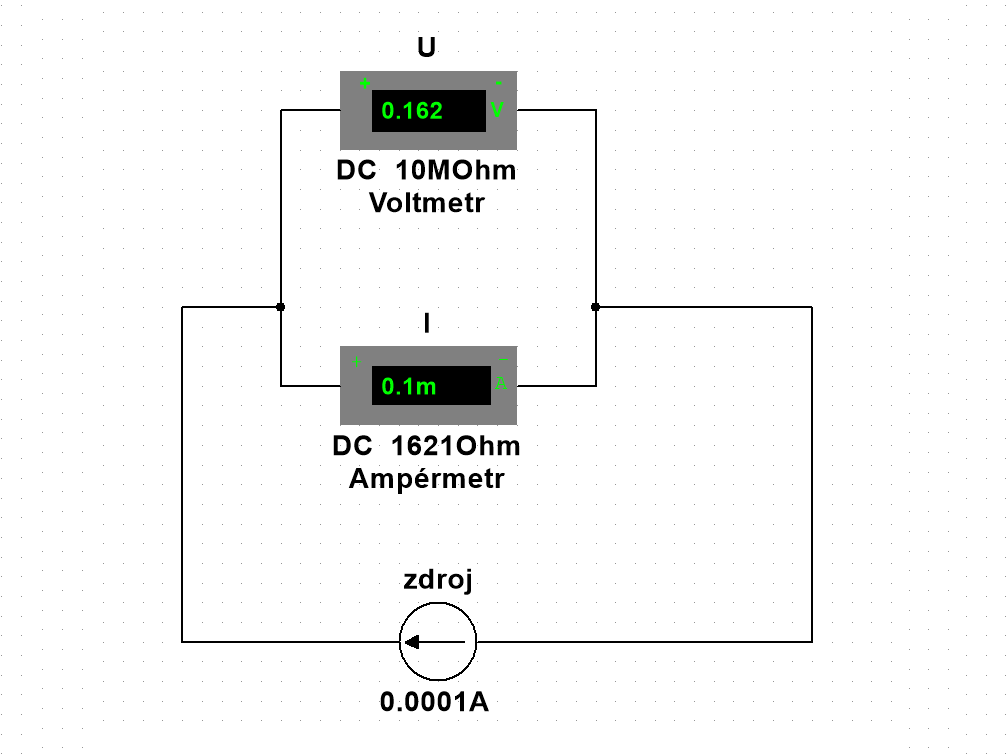
\includegraphics[width=0.85\textwidth,]{Odpor pres Voltmetr}
							\caption {Vizualizace zapojení a simulace získaných hodnot v počítačovém programu MultiSim}
							
			\end{center}
		\end{figure}
		Proto vnitřní odpor ampérmetru získáme vztahem
		\begin{equation}
			R = \frac{U_V}{I_A}
		\end{equation}
		Kde $U_V$ je napětí měřené voltmetrem a $I_A$ proud měřený ampérmetrem.
		
		
		Při použití odporové dekády využíváme skutečnosti, že je proud protékající dvěma větvemi - je-li jejich odpor stejný - rozdělen přesně na poloviny. Z prvního Kirchhofova zákona víme, že divergence proudu v uzlu je nulová, nulová je tedy suma všech proudů (při respektování jejich směrů), tj. kolik "přiteče" \, tolik i "odteče". Zároveň víme, že každá větev musí podléhat pravidlům Ohmova zákona, a pokud Komponenty na každé z větví uvažujeme jako rezistory (skutečnost, že uvažujeme cívku v~ručkovém ampérmetru jako rezistor měření vnitřního odporu negativně neovlivní, jelikož nás zajímají právě odpory na uvedených větvích, nic jiného) nás dovede k závěru, že každou z větví musí protékat právě poloviční proud. Z tohoto vyčerpávajícího textu tedy můžeme sestavit méně vyčerpávájící formule:
		\begin{gather*}
			\sum_{i=1}^{n} = 0 \\
			I_1 - I_2 -I_3 = 0 \\
			{I_1 = I_2 + I_3} \\
			I_1 = \frac{U}{R} + \frac{U}{R} = \frac {2U}{R} \\
			\frac{I_1}{2} = \frac{U}{R} = I_2 = I_3
		\end{gather*}
		Kde $I_1, I_2, I_3$ jsou proudy na jednotlivých větvích a $U$ úbytek napětí na rezistorech (z 2. K.z. víme, že se při paralelním zapojení musí rovnat) a $R$ jsou odpory na větvi 2 a 3. Jak vidíme, tak se při stejném odporu obou větví $2, 3$ jejich proudy rovnají \textbf{a zároveň jsou poloviční vůči $I_1$}.
		\begin{figure}[h]\begin{center}
				
			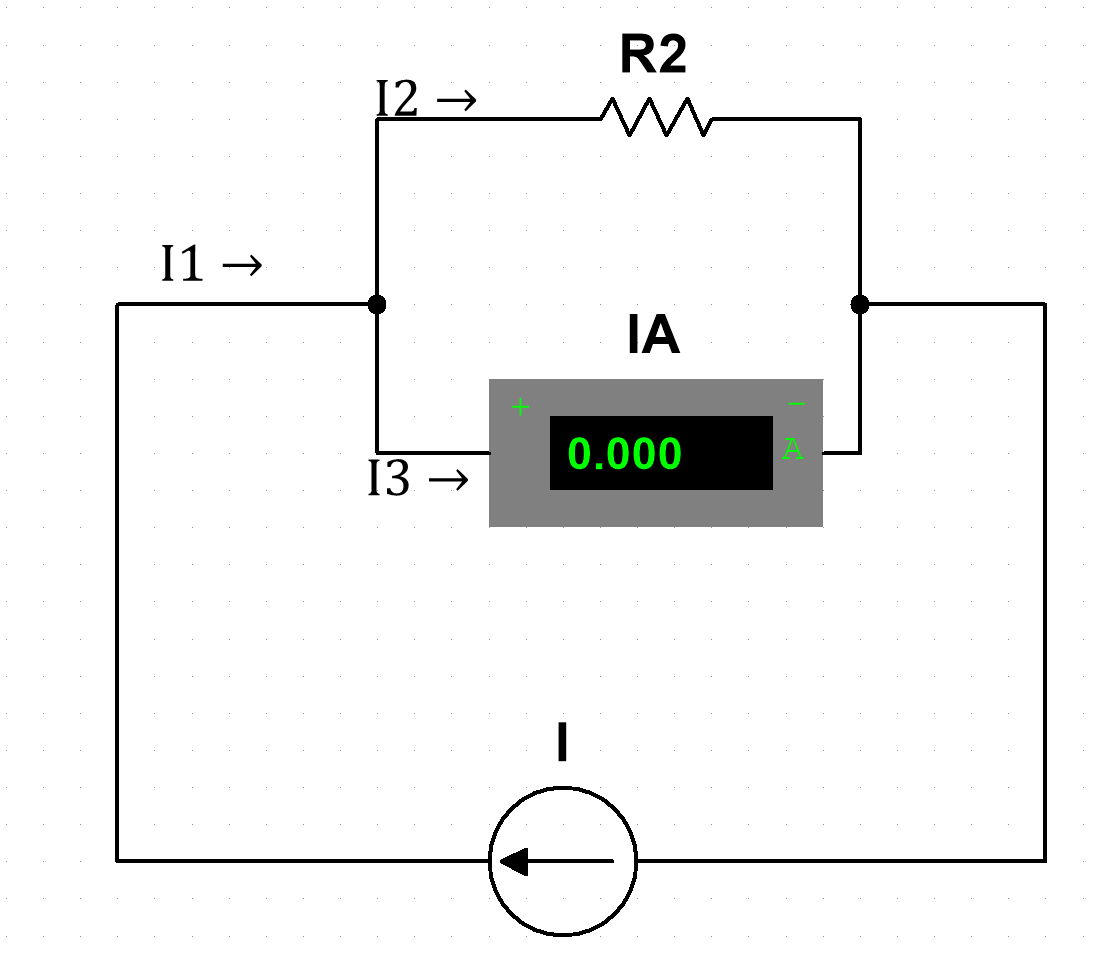
\includegraphics[width=0.45\textwidth,]{vetev realizovana}
			\includegraphics[width=0.45\textwidth,]{vetev}
			\end{center}
		\end{figure}
		Proto k měření vnitřního odporu ampérmetru můžeme využít odporové dekády a odpor na dekádě upravit, aby proud na ampérmetru vůči zapojení bez dekády dosáhl poloviční hodnoty. V takové situaci totiž musí platit, že se odpor dekády rovná odporu ampérmetru, \textbf{čímž získáváme informaci o jeho vnitřním odporu}. Pro vnitřní odpor získáváme první metodou $R_A = 1597 \pm 20 \,\rm \Omega$, druhou metodou $R_A = 1621 \pm 20 \,\rm \Omega$
		
		\subsubsection{Zvětšení rozsahu ampérmetru}
		Zde budeme využívat principů popsaných při měření vnitřního odporu dekádou - tu využijeme na dělení proudu mezi větvemi 2-3, čímž můžeme zvýšit rozsah ampérmetru, jelikož větví, ve které je umístěn, bude protékat pouze část proudu, který obvodem protéká. Formuli si znovu můžeme odvodit, využijeme skutečnosti, že úbytek napětí na paralelních větvích se musí rovnat:
		\begin{gather*}
			R_3 I_3 = R_2 I_2\\
			\text{využijeme skutečnosti, že dle I. K.z. platí}\, I_3 = I_1 - I_2 \\
			R_3 (I_1 - I_2) = R_2 I_2 \\
			R_3 = \frac{R_2}{\frac {I_1} {I_2} -1} \\
			R_o = \frac{R_A}{\frac{I_N}{I_A}-1}
		\end{gather*}
		Znovu vycházíme z nákresu uzlu a větví výše. Proud $I_2$ protékající ampérmetrem nesmí v žádném zapojení přesáhnout maxima rozsahu ampérmetru. Proud $I_1$, tj celkový proud protékající smyčkou, však při dostatečné změně odporu dekády smí být vyšší. Odpor dekády spočítáme formulí odvozenou výše, kde $R_3$ resp. $R_o$ je odpor dekády, $R_2$, resp. $R_A$ odpor ampérmetru, $I_N (I_1)$ je nový maximální proud protékající obvodem a $I_A (I_2)$ původní maximální proud definovaný rozsahem ampérmetru.
		Pro zvětšení rozsahu získáváme hodnoty:
		\begin{align*}
			0.5 \text{ mA}: R_o = 399 \pm 6 \text{ $\Omega$} \\
			1 \text{ mA}: R_o = 177.4 \pm 2.7 \text{ $ \Omega$} \\
			2 \text{ mA}: R_o = 74.0 \pm 1.3 \text{ $ \Omega$} 
		\end{align*}
		Při odpovídajících odporech zvyšujeme postupně proud zdroje a vidíme, že se rozsah skutečně zvýšil na správné hodnoty.
		
		\subsubsection{Použití ampérmetru jako voltmetr a změna jeho rozsahu}
		Z Ohmova zákona vyplývá, že známe-li proud protékající ampérmetrem a zároveň jeho vnitřní odpor, jednoduše získáme úbytek napětí na ampérmetru. Nicméně je znovu nutno dbát na maximální rozsah ampérmetru a pokud chceme dosáhnout smysluplného odečtení hodnot rovnou z ručkového ampérmetru bez dalších výpočtů, bude znovu potřeba jeho rozsah nějak upravit. S vnitřním odporem cca 1620 Ohm totiž v souladu s O.z (tj. $U = RI$) bude maximální rozsah námi stvořeného voltmetru 0.1621 V, což je hodnota poměrně nepraktická. Chceme být schopni přístroj upravit tak, aby hodnoty odečtené z~něj byly jednoduše konvertibilní na reálné hodnoty a zároveň zvýšit rozsah přístroje (aby nám tedy přístroj při rozsahu 5V ukazoval maximum své škály.) Tohoto efektu získáme realizací úbytku napětí před voltmetrem.
		Pro ampérmetr (voltmetr) musí platit Ohmův zákon, kterým získáme maximální úbytek napětí, které na voltmetru smí nastat:
		\begin{equation}
			U_m = R_A I_m
		\end{equation}
		kde $I_m$ je maximální proud protékající ampérmetrem (def. rozsahem) $R_A$ vnitřní odpor ampérmetru a $U_m$ maximální úbytek napětí. Při zapojení zdroje o libovolném napětí $U$ a odporové dekády, která nám dostatečný úbytek napětí $U_o$ realizuje, bude platit:
		\begin{equation}
			U = U_o + U_m.
		\end{equation} Vztah můžeme odvodit znovu velmi jednoduše a podobně jako v případě zvýšení rozsahu ampérmetru, využíváme skutečnosti, že proud protékající dekádou i ampérmetrem se bude rovnat.
		\begin{gather*}
			I = I \\
			\frac{U_o}{R_o} = \frac{U_m}{R_A} \\
			\frac{R_o}{U_o} = \frac{R_A}{U_m} \\
			\frac{R_o}{U - U_m} = \frac 1 {U_m} R_A \\
			R_o = \frac{U - U_m}{U_m}R_A \\
			R_o = \left(\frac{U}{U_m} -1\right) R_A\\			
			R_o = \left(\frac{U}{I_m R_A} -1\right) R_A\\			
			R_o = \frac{U}{I_m} - R_A
		\end{gather*} Získáváme tedy formuli, pomocí které zjistíme, jaký odpor dekády $R_o$ nastavit, aby ručka voltmetru byla na svém maximu při napětí $U$, tedy novém rozsahu. Pro rozsah 5V a 10V získáváme hodnoty odporu:
		\begin{align*}
			5 \text{ V}: R_o = 48 400 \pm 20 \text{ $\Omega$} \\
			10 \text{ V}: R_o = 98400 \pm 20 \text{ $ \Omega$} 
		\end{align*} Znovu vidíme, že při odpovídajícím nastavení odporu na dekádě můžeme napětí na zdroji zvyšovat až k maximu rozsahu.

   \subsection{Digitální část}
   \subsubsection{Číselný rozsah D/A převodníku}
   Převodník o \textbf{$n$} bitech nám dokáže realizovat hodnoty ve dvojkové soustavě, přičemž při konverzi vidíme, že kupř. 8-bit převodník realizuje hodnoty $K K K K K K K K$, kde $K$ je 0 nebo 1. Zároveň každý z bitů při hodnotě 1 vytváří číslo $2^(n-i)$, kde n je celkový počet bitů a i je pořadí hodnoty (zleva doprava) začínající nulou. Celková hodnota, jsou-li veškeré bity ve stavu 1, tedy budou vypadat následovně: $2^7 + 2^6 + 2^5 + 2^4 + 2^3 + 2^2 + 2^1 + 2^0$, což lze zapsat jako $2^8 -1$. Rozsah převodníků o libovolném počtu bitů můžeme získat prostřednictvím formule $2^n -1$, kde n je znova počet bitů. Maximální hodnota 8-bitového převodníku je tedy 255 (vidíme zde do očí bijící korelaci s osmibitovými barevnými kanály, které mají též hodnoty 0-255). U 16-bit převodníku máme rozsah 0 - 65 535.
   
   \subsubsection{Napěťový rozsah D/A převodníku}
   Zde počítáme napěťový rozsah pro osmibitový a šestnáctibitový modul - měříme hodnoty napětí při vstupních hodnotách v celém rozsahu, hodnoty vykreslíme do grafů.
   
  	 \begin{figure}[H]\begin{center}
  	 		
   	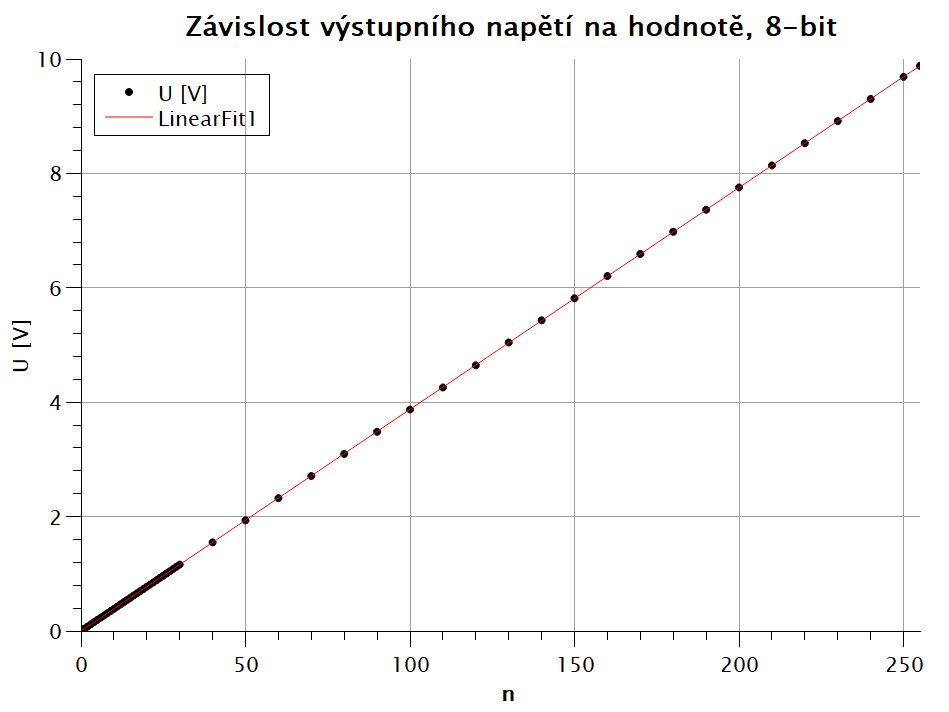
\includegraphics{8bitzavislost}
   	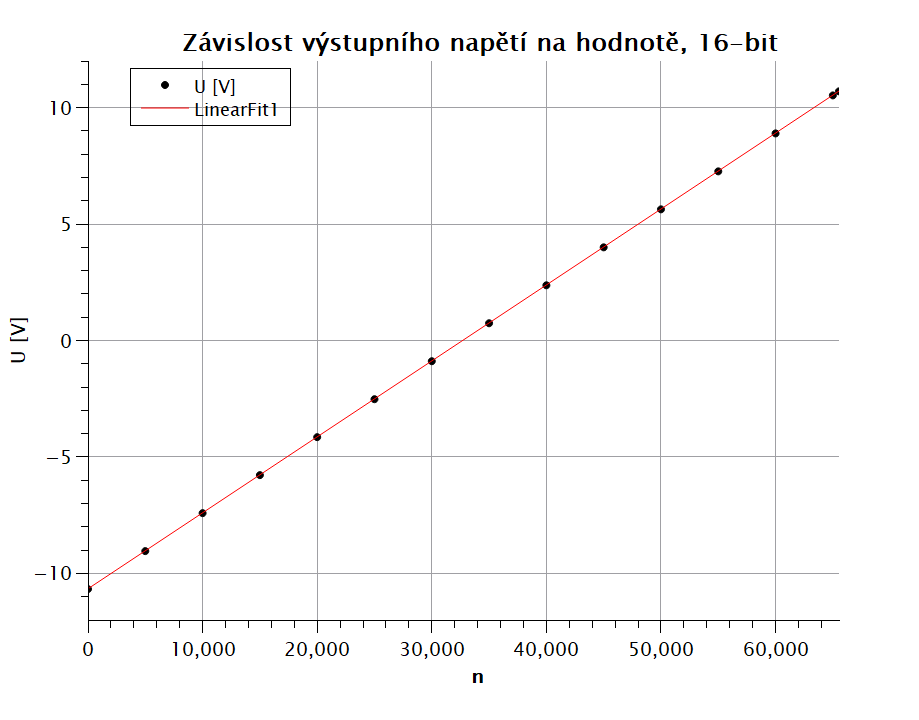
\includegraphics{16bitzavislost}
  	 	\end{center}
   \end{figure}
    \noindent Ze získaných hodnot vidíme, že rozsah 8-bit převodníku je\\ $U_{min} = 0.001264 \pm 1.3.10^{-5} \,\rm V$, $U_{max} = 9.88 \pm 0.002 \,\rm V$ \\ u 16-bit je rozsah  \\ $U_{min} = -10.674 \pm 0.002 \,\rm V$, $U_{max} = 10.697 \pm 0.002 \,\rm V$
	\subsubsection{Vliv vzorkovací frekvence na kvalitu záznamu analogového signálu}
	Harmonický signál o frekvenci 1kHz zaznamenáváme A/D převodníkem a v měřícím systému ISES jej zaznamenáváme s různými vzorkovacími frekvencemi (20kHz-100Hz). Po vizuální kontrole získaných dat vidíme, že nám harmonický signál zaznamenají pouze frekvence 20kHz, 2kHz a 1.1kHz, tedy frekvencí větších, než je samotná frekvence signálu. U 1.1kHz ale vidíme, že zaznamenaný harmonický signál \textbf{neodpovídá} vysílanému signálu, místo něj měříme signál o frekvenci 100Hz, tj. rozdílu frekvence signálu a frekvence vzorkovací. Vidíme, že vzorkovací frekvence musí být alespoň dvakrát vyšší, než frekvence signálu, abychom zaznamenávali skutečná data. \textit{Právě proto je standardní vzorkovací frekvencí u nahrávání zvuku 44.1, resp. 48kHz; zachytí nám totiž frekvence až do hodnot 22, resp. 24 kHz, což jsou právě frekvence na prahu rozsahu lidského slyšení. (Kdyby si delfíni rozjeli audioprůmysl, museli by nahrávat se vzorkovací frekvencí zhruba 400kHz, což by generovalo soubory o velmi nepříjemných velikostech (cca 10x větší, než ty naše)).}
	
	\section{Závěr}
	Podařilo se nám změřit vnitřní odpor ampérmetru metodou odporové dekády i digitálního voltmetru. Tuto informaci jsme dokázali utilizovat pro zvětšení rozsahu ampérmetru i následného využití přístroje jako voltmetr. U digitální části jsme vypočítali číselné rozsahy převodníků, zopakovali si základy \textbf{milované} dvojkové soustavy (někde mi tu v šuplíku leží hodinky ukazující čas právě v ní), změřili jsme napěťové rozsahy převodníků a psychicky se připravili na předmět kmity-vlny-optika při zjišťování vlivu vzorkovací frekvence na kvalitu záznamu signálu. 

	% Nakonec nezapomeňte projet text programem vlna nebo vlnka, např.
	% 	vlna -m -l -n mojeuloha.tex
	% nebo zkontrolovat a opravit jednopísmenné předložky na koncích řádků ručně.
	
	
\end{document}
